\documentclass[25pt, a0paper, portrait]{tikzposter}
\usepackage[T1]{fontenc}
\renewcommand*\familydefault{\sfdefault}
\usepackage{sfmath}
\usepackage{amsmath}
\usepackage{lipsum}
\usepackage[compress]{cite}
\usepackage{verbatim}

\newcommand{\prd}{PRD}
\newcommand{\prr}{PRR}
\newcommand{\mnras}{MNRAS}
\newcommand{\jcap}{JCAP}
\newcommand{\jmap}{JMAP}
\newcommand{\joss}{JOSS}
\newcommand{\pasa}{PASA}
\newcommand{\aap}{A\&A}
\newcommand{\prl}{PRL}
\newcommand{\arxiv}{arXiv}

\makeatletter
\renewcommand\TP@maketitle{%
    \centering
    \vspace{-40pt}
    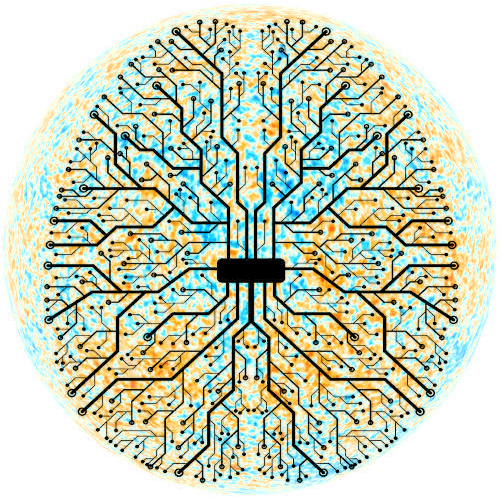
\includegraphics[height=0.11\textwidth]{handley-lab.png}\hfill
    \begin{minipage}[b]{0.7\linewidth}
        \centering
        \color{titlefgcolor}
        {\Huge \sc \@title \par}
        \vspace*{1em}
        {\huge \@author \par}
        \vspace*{1em}
        {\LARGE \@institute}
    \end{minipage}%
    \hfill
\includegraphics[height=0.11\textwidth]{cambridge-cropped.pdf}
}
\makeatother

\title{Bayesian Anomaly Detection for Ia Supernovae using JAX-bandflux}
\author{Sam Leeney, Will Handley, Harry Bevins, Eloy de Lera Acedo}
\institute{Kavli Institute for Cosmology $\cdot$ Cavendish Laboratory $\cdot$  University of Cambridge}

\usetheme{Envelope}

\tikzposterlatexaffectionproofoff{}

\let\oldbibliography\thebibliography
\renewcommand{\thebibliography}[1]{\oldbibliography{#1}
\setlength{\itemsep}{-5pt}}

\pdfinclusioncopyfonts=1


\begin{document}
\maketitle

\block{}{%
    \centering
    
\includegraphics[height=0.075\textwidth]{kicc.png}
    \hspace{20pt}
    \begin{minipage}[b]{0.73\textwidth}
        \centering
        \textbf{Robust parameter estimation for Type Ia supernovae is crucial for precision cosmology.} Anomalous data points from instrumental artifacts or astrophysical contamination can bias SALT3 fits and propagate into cosmological parameters. We present a differentiable Bayesian framework that simultaneously fits supernova light curves while identifying anomalous observations, implemented in JAX for GPU acceleration.
    \end{minipage}%
    \hspace{20pt}
    \includegraphics[height=0.075\textwidth]{headshot.jpg}
}

\begin{columns}
    \column{0.5}

    \block{Bayesian Anomaly Detection}{%
        \textbf{Problems with current methods:}
        \begin{itemize}
            \item Traditional methods are not model aware
            \item Anomalies sought before/after fitting, not simultaneously
            \item Binary classification (no encoding of belief)
            \item Standard likelihoods cannot incorporate anomalous data
        \end{itemize}
        
        \vspace{0.2em}
        \textbf{Our solution}
        
        \vspace{0.2em}
        We model each data point as either expected or anomalous:
        
        \textbf{1. Define anomaly mask:} $\varepsilon_i \in \{0, 1\}$ for each data point
        
        \textbf{2. Bernoulli prior:} $P(\varepsilon_i) = p^{\varepsilon_i}(1-p)^{(1-\varepsilon_i)}$
        
        \textbf{3. Piecewise likelihood:}
        \begin{equation}
            P(\vec{D}, \vec{\epsilon} | \theta) = \prod_{i=1}^{N} \left(L_i(\theta) (1-p)\right)^{(1-\epsilon_i)} \left(\frac{p}{\Delta}\right)^{\epsilon_i}
            \nonumber
        \end{equation}
        
        \textbf{4. Marginalize over $\epsilon$:} $P(\mathcal{D} | \theta) = \sum_{\varepsilon \in \{ 0, 1 \} ^N}P(\mathcal{D},\varepsilon|\theta)$
        
        \textbf{5. Dominant mask approximation:}
        \begin{equation}
            P(\mathcal{D}|\theta, \varepsilon_{\mathrm{max}}) \gg \mathrm{max}_j P(\mathcal{D}|\theta,\varepsilon^{(j)})
            \nonumber
        \end{equation}
        
        \textbf{6. Final log-likelihood:}
        \begin{equation}
        \log P(\mathcal{D}|\theta) =
        \begin{cases}
        \log \mathcal{L}_i + \log(1 - p), & \text{if } \log \mathcal{L}_i + \log(1 - p) > \log p - \log \Delta \\
        \log p - \log \Delta, & \text{otherwise}
        \end{cases}
        \nonumber
        \end{equation}
        
        \vspace{0.3em}
        \innerblock{Key Insight}{%
            We fit for this 'floor' as a free parameter, fully automating the
            anomaly detection process.
        }
        
        \vspace{0.3em}
        \textbf{Demo:} \\
        {\small github.com/samleeney/Bayesian-Anomaly-Detection/blob/main/demo\_anomaly\_detection.ipynb}
        
        \vspace{0.3em}
        \centering
        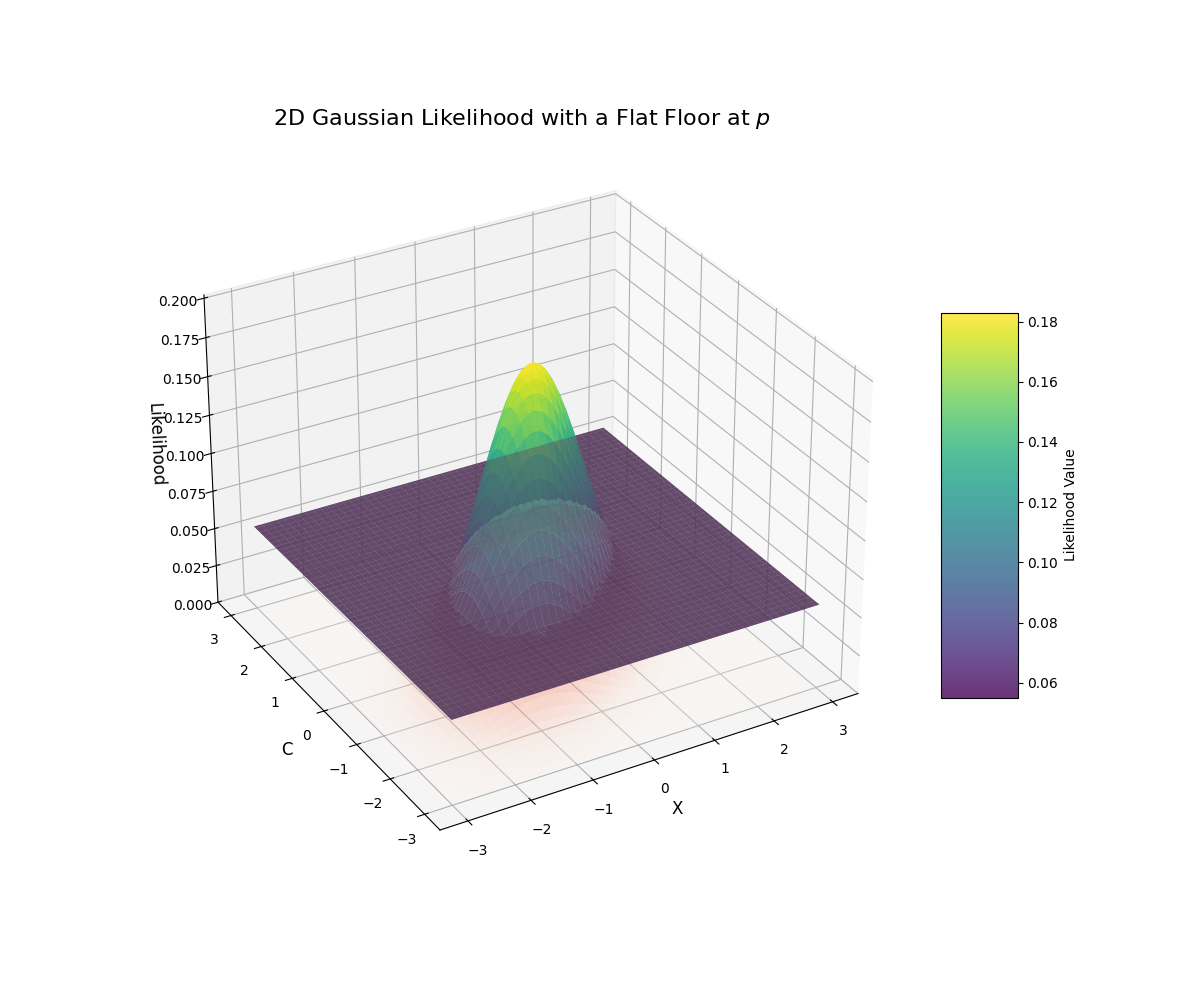
\includegraphics[width=0.75\linewidth]{likelihood_floor_plot.png}
    }
    
    \block{SN 19amo: Light Curve}{%
        \centering
        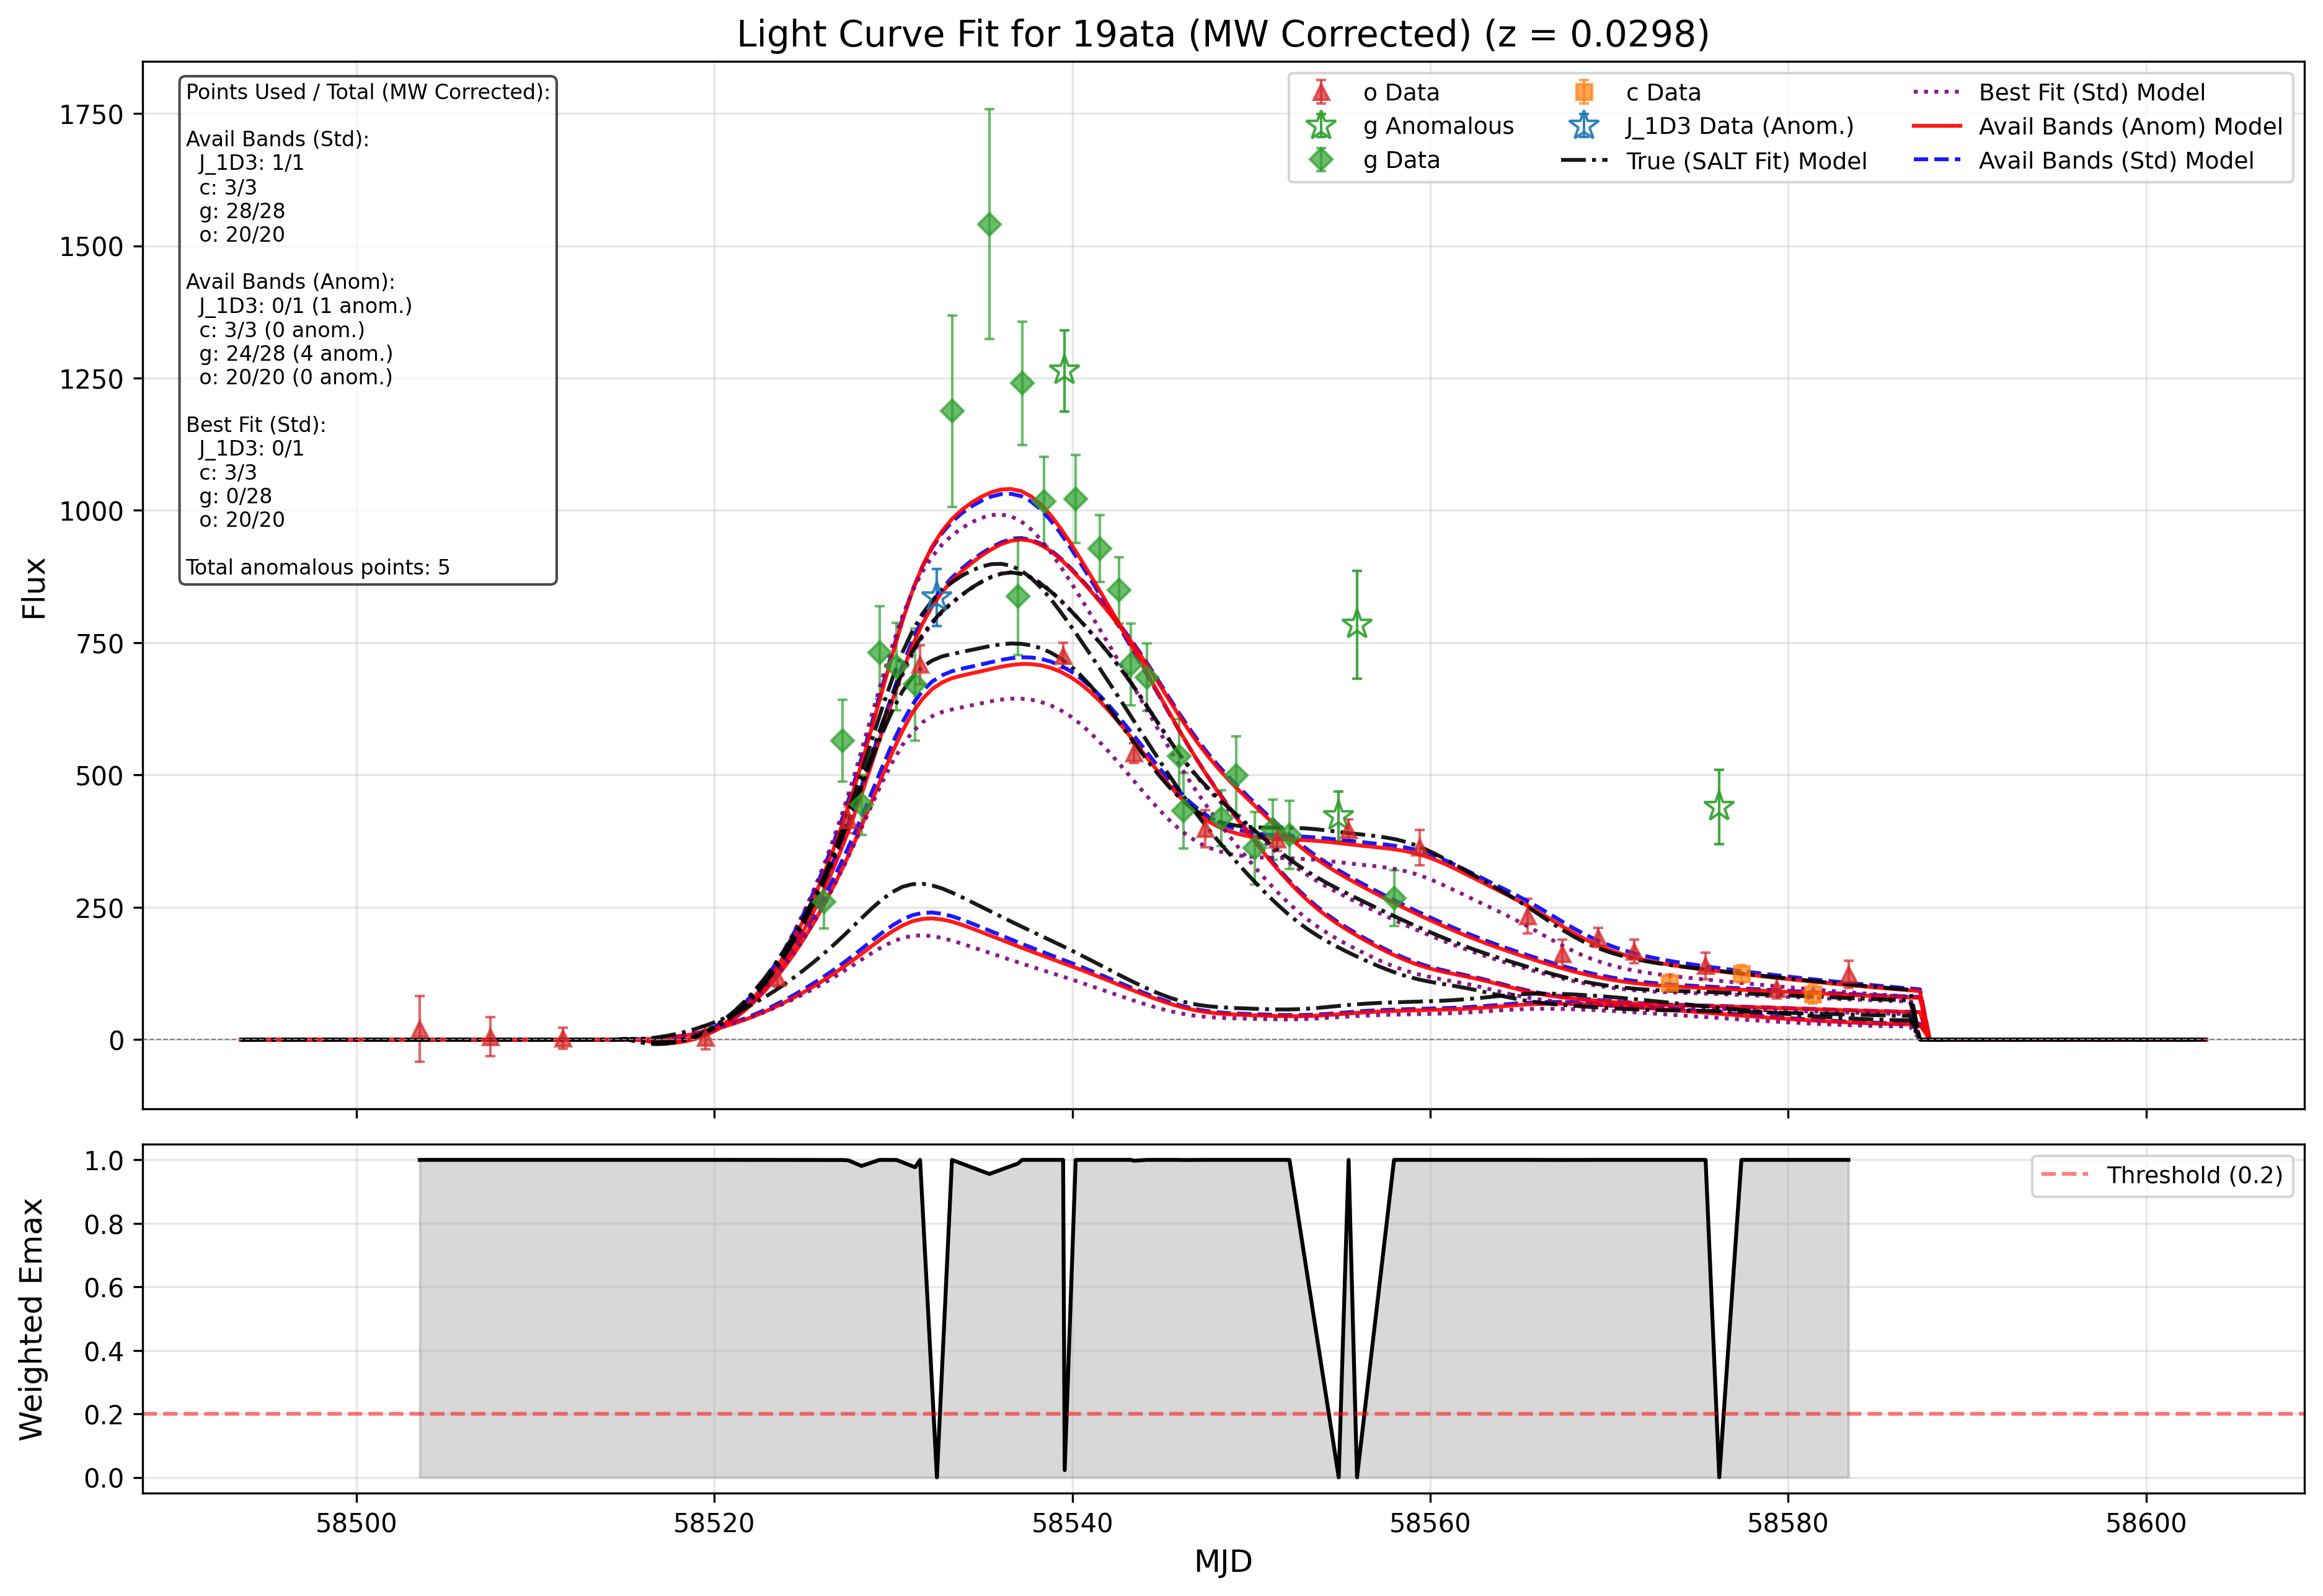
\includegraphics[width=0.8\linewidth]{light_curve_comparison_19amo.png}
        
        \vspace{0.2em}
        {\small Data from Do et al. (2025)}
    }

    \column{0.5}

    \block{JAX-bandflux}{%
        \textbf{A differentiable framework for supernova analysis:}
        
        \textbf{Key Features:}
        \begin{itemize}
            \item GPU-accelerated SALT3 model fitting
            \item Built on JAX for automatic differentiation
            \item Integrates with BlackJAX for nested sampling
            \item Handles large supernova datasets efficiently
        \end{itemize}
        
        \vspace{0.5em}
        \textbf{Example:} handley-lab.co.uk/nested-sampling-book/physics/supernovae.html
        
        \vspace{0.5em}
        \textbf{SALT3 Model:}
        \begin{equation}
            F(p, \lambda) = x_0 \left[M_0(p, \lambda) + x_1M_1(p, \lambda)\right] \times e^{c \times CL(\lambda)}
            \nonumber
        \end{equation}
        
        \textbf{Bandflux Integration:}
        \begin{equation}
            F_{\text{band}} = \int_{\lambda_{\text{min}}}^{\lambda_{\text{max}}} F(p, \lambda) \cdot T(\lambda) \cdot \frac{\lambda}{hc} d\lambda
            \nonumber
        \end{equation}
        
        \vspace{0.5em}
        \begin{center}
            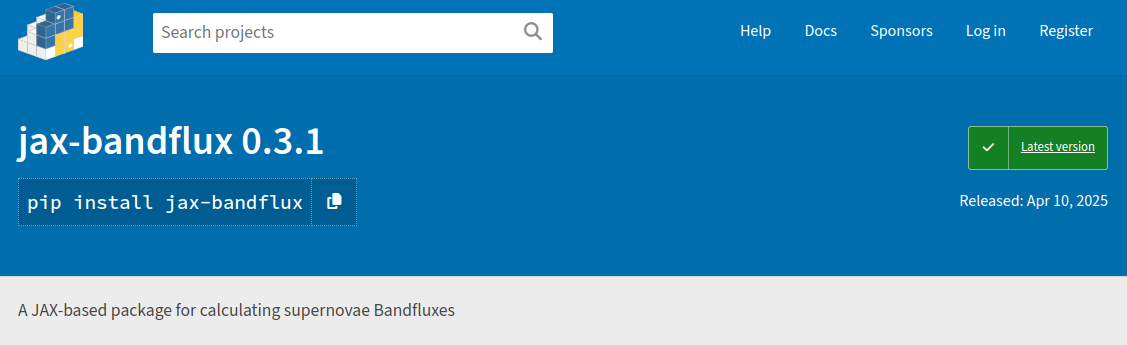
\includegraphics[width=0.55\linewidth]{pip-jax-bandflux.png}
            \hspace{0.5em}
            
\includegraphics[width=0.25\linewidth]{jax_logo_250px.png}
        \end{center}
    }
    
    \block{Main Advantages}{%
        \textbf{Utility of Bayesian anomaly detection for Ia analysis:}
        \begin{enumerate}
            \item Fully automated anomaly detection
            \item Fully automated filter selection
            \item Preserves previously 'bad' filters by mitigating anomalies  
        \end{enumerate}
    }
    
    \block{Corner Plot Comparison}{%
        \centering
        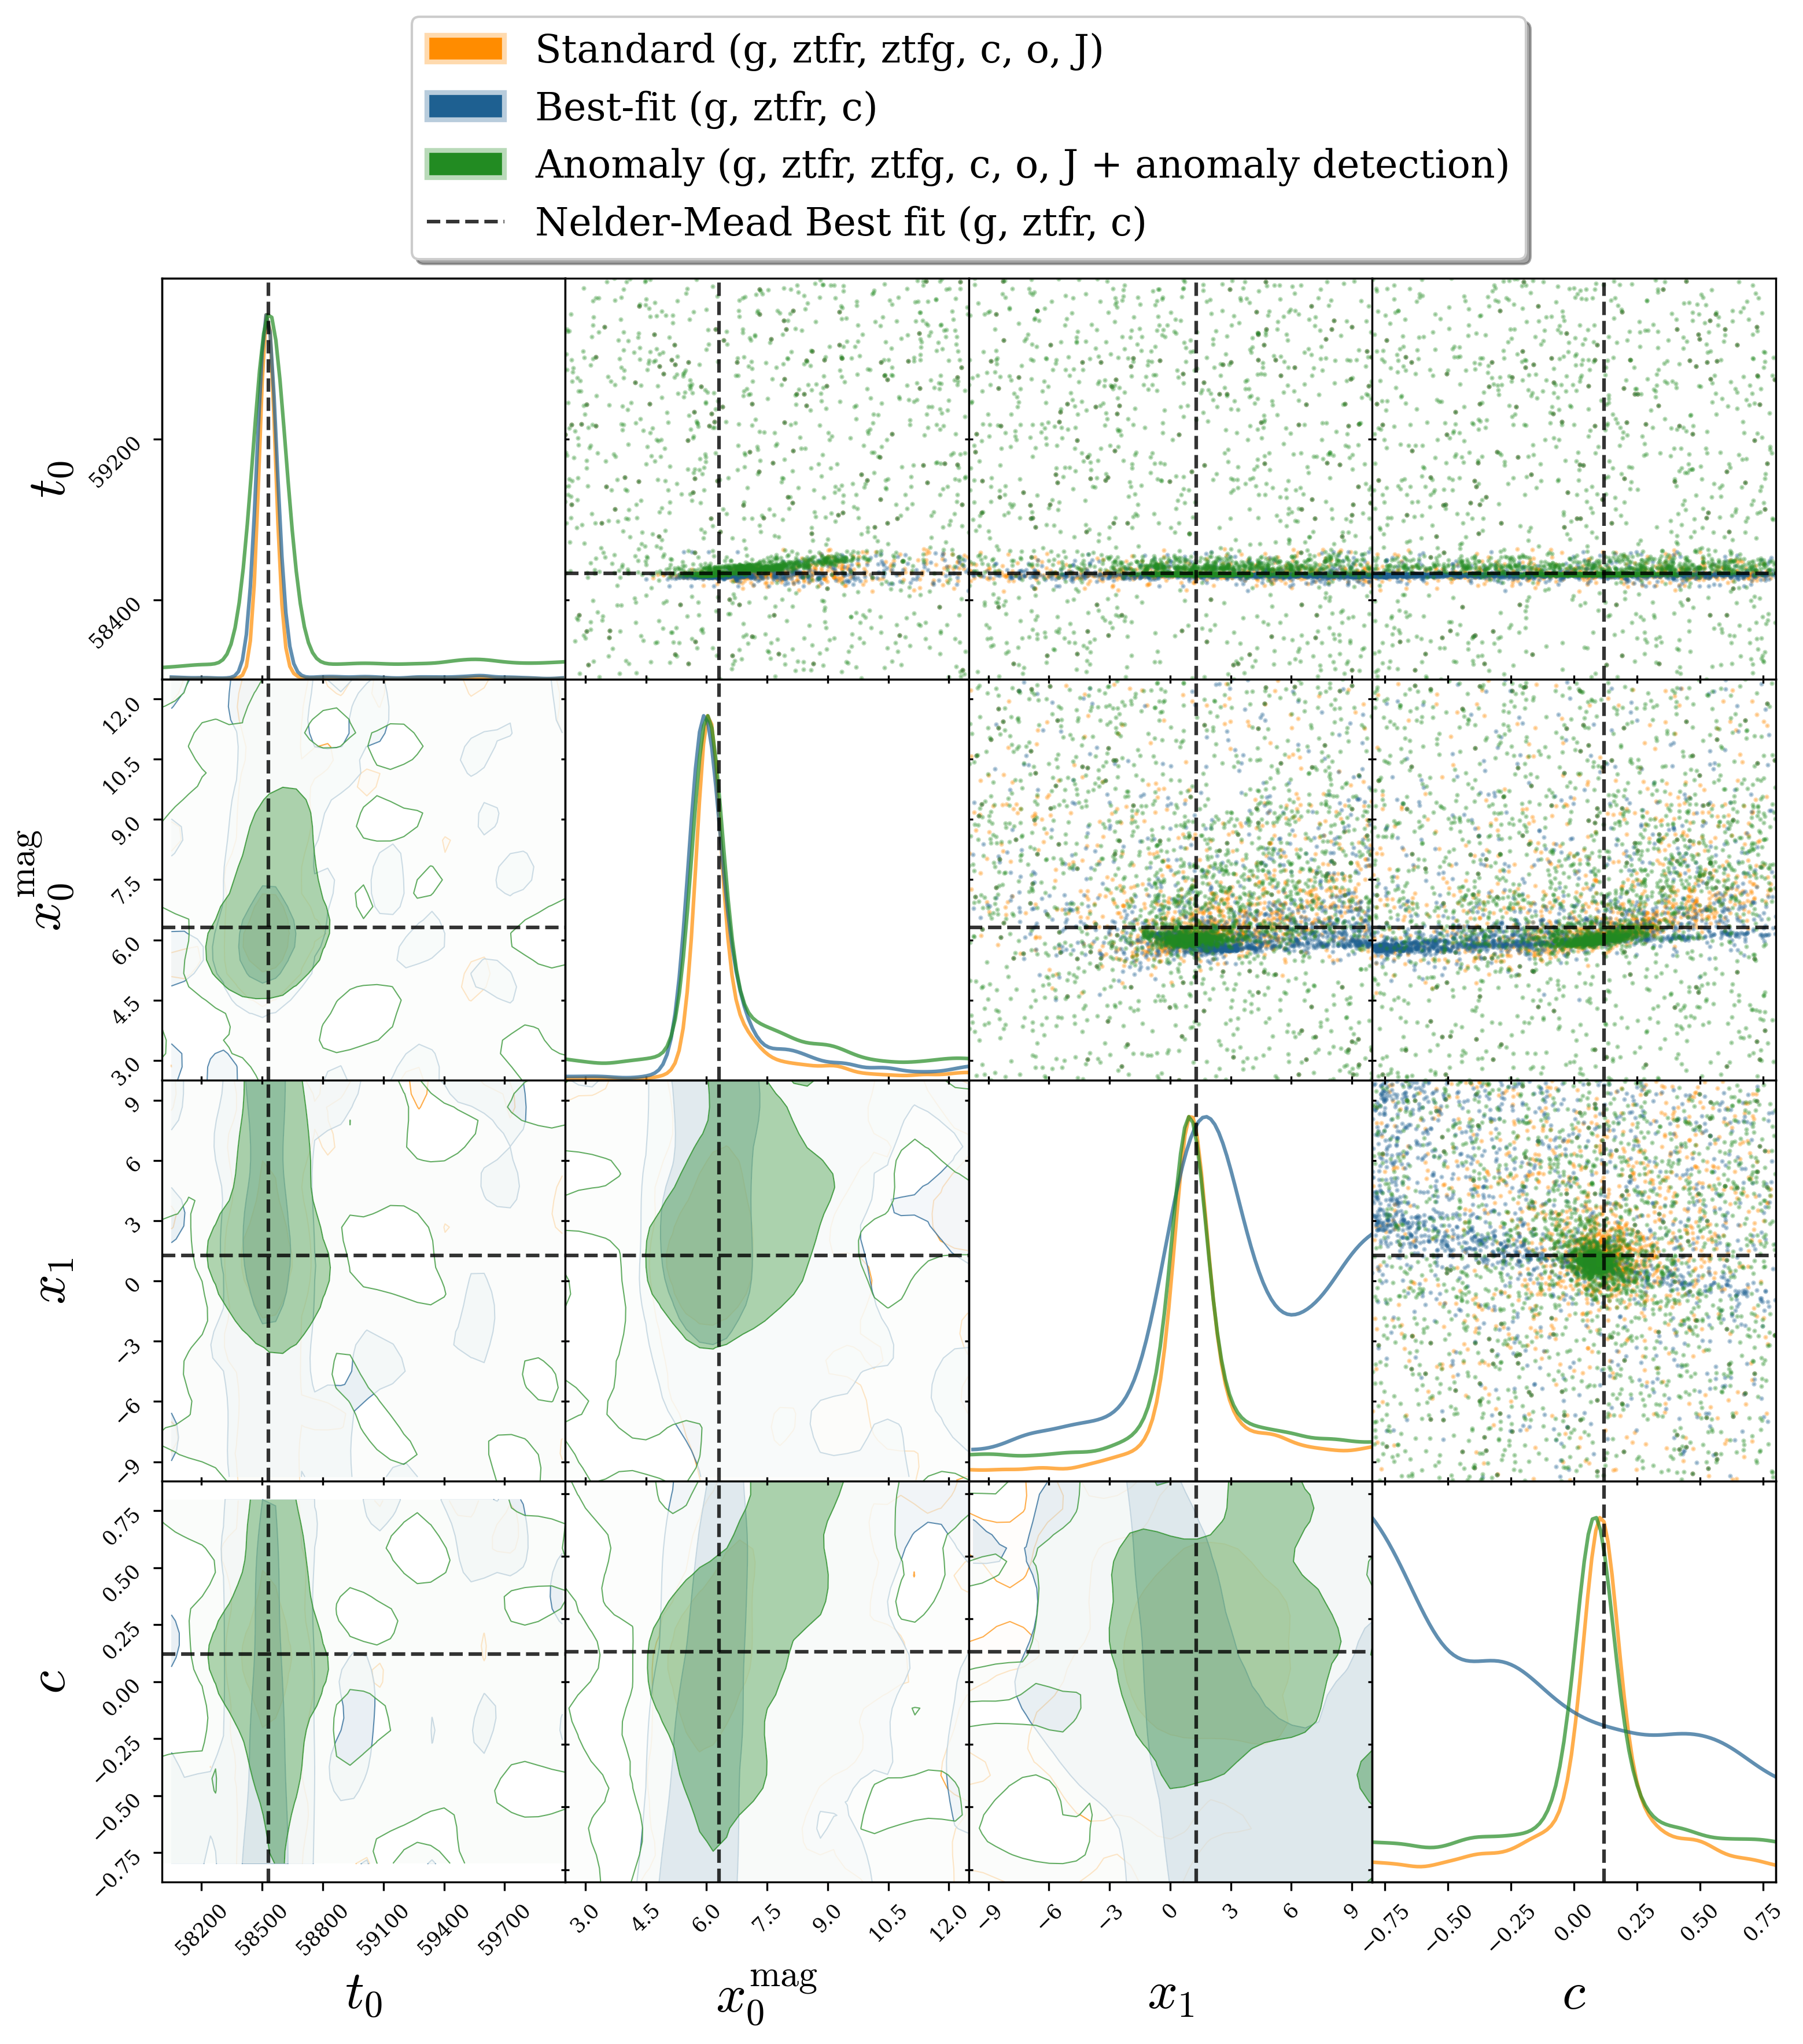
\includegraphics[width=0.62\linewidth]{corner_comparison.png}
        
        \vspace{0.1em}
        {\small Standard SALT (orange) vs. anomaly detection (green) - tighter constraints.}
    }
    
    \block{Next Steps}{%
        \begin{minipage}[t]{0.75\linewidth}
            \vspace{0pt}
            \textbf{Future Applications:} 
            \begin{itemize}
                \item Extend framework for distance measurements
                \item Estimate H$_0$ using robust supernova samples
                \item Apply to other astronomical datasets
            \end{itemize}
            
            \vspace{0.1em}
            \textbf{Code:} github.com/samleeney \\
            \textbf{Paper:} arXiv:2211.15448
        \end{minipage}%
        \hfill
        \begin{minipage}[t]{0.2\linewidth}
            \vspace{0pt}
            \centering
            
\includegraphics[width=1.0\linewidth]{qr.png}
        \end{minipage}
    }
    
\end{columns}

\end{document}
